\documentclass[a4paper,11pt,twocolumn]{article}

\usepackage{aas_macros}

\usepackage[utf8]{inputenc}
\usepackage[T1]{fontenc}
\usepackage{lmodern}
%\usepackage{times}
%\usepackage[margin=2cm]{geometry}
\usepackage[a4paper]{geometry}
\usepackage{amsmath}
\usepackage{mathtools}
\usepackage{graphicx}
\usepackage{multirow}
\usepackage{blindtext}
\usepackage{hyperref}
\usepackage{float}

\usepackage{pgfplotstable}
\usepackage{booktabs}
% \pgfplotsset{compat=1.18}


\graphicspath{ {./images/} }

\usepackage[czech]{babel}
\usepackage{graphicx}
\usepackage{amsmath}
\usepackage{xspace}
\usepackage{url}
\usepackage{siunitx}
\usepackage{indentfirst}
\usepackage{subcaption}
\usepackage{caption}
\usepackage{tabularx}
\usepackage{rotating}
\usepackage{tikz}
\usepackage[labelformat=parens,labelsep=quad,skip=3pt]{caption}

\usepackage{color}
\usepackage{listings}

\definecolor{codegreen}{rgb}{0,0.6,0}
\definecolor{codegray}{rgb}{0.5,0.5,0.5}
\definecolor{codepurple}{rgb}{0.58,0,0.82}
\definecolor{backcolour}{rgb}{0.95,0.95,0.92}

\lstdefinestyle{mystyle}{
    backgroundcolor=\color{backcolour},
    commentstyle=\color{codegreen},
    keywordstyle=\color{magenta},
    numberstyle=\tiny\color{codegray},
    stringstyle=\color{codepurple},
    basicstyle=\ttfamily\footnotesize\centering,
    breaklines=true,
    captionpos=b,
    numbers=left,
    numbersep=5pt,
    showspaces=false,
    showstringspaces=false,
    showtabs=false,
    tabsize=2
}

\lstset{style=mystyle}

%\widowpenalty 10000 \clubpenalty 10000 \displaywidowpenalty 10000
\setcounter{topnumber}{3}
\setcounter{bottomnumber}{3}
\setcounter{totalnumber}{6}
\renewcommand\topfraction{0.9}
\renewcommand\bottomfraction{0.9}
\renewcommand\textfraction{0.1}
\intextsep=8mm \textfloatsep=8mm

\renewcommand{\thesection}{\arabic{section}.}
\renewcommand{\thesubsection}{\thesection\arabic{subsection}.}
\makeatletter \def\@seccntformat#1{\csname the#1\endcsname\hspace{1ex}} \makeatother


\begin{document}
    \twocolumn[
    \noindent\hrulefill
    \begin{center}
        \bigskip
        \huge Radiální rychlost z analýz telurických čar
        \vspace{0.2cm}
        \par \large F4191: Praktikum z astronomie 2
        \par \large Artem Gorodilov
        \vspace{0.2cm}
        \par \large 20. ~prosince 2024
        \bigskip
    \end{center}
    \noindent\hrulefill
    \bigskip
    ]

    \vskip10pt
    \section{Abstrakt}
        V této práci jsem analyzoval tři spektra. Dvě z nich patřila stejnému objektu FVSco a jedno objektu HD64740. Spektrum FVSco-04\_44.fits byl získán pomocí dalekohledu ESO 1.52 s expoziční dobou 1800 s. Spektrum FVSco-209\_06.fits byl získán přístrojem FEROS umístěným na dalekohledu MPG/ESO 2.2, expoziční doba 800 s. Spektrum HD64740\_010r\_26.wl.fits byl získán přístrojem HARPS namontovaným na dalekohledu ESO 3.6. 
        
        Všechna pozorování byla provedena na observatoři La Silla.
        
        Výpočty byly provedeny pomocí skriptu v Pythonu\textsuperscript{\cite{github}}.
    \section{Úvod}
        Tellurické čáry ve spektru jsou absorpční čáry způsobené molekulami v zemské atmosféře, jako je kyslík, voda nebo oxid uhličitý. Tyto čáry se objevují ve spektru hvězd, když světlo prochází atmosférou Země, a jejich poloha je pevně vázána na radiální rychlost pozorovatele vůči Zemi.

        Pro určení radiální rychlosti je možné porovnat spektrum hvězdy s tellurickými čarami. Protože tyto čáry mají známou a stabilní vlnovou délku, slouží jako referenční body. Posun hvězdných čar vůči tellurickým pak lze využít k měření Dopplerova posuvu, a tím i k určení radiální rychlosti hvězdy.
        
        Tato metoda je obzvláště užitečná v infračerveném oboru spektra, kde jsou tellurické čáry výrazné, ale vyžaduje přesnou kalibraci a modelování, aby byly atmosférické vlivy správně odstraněny.

        Radiální rychlost $\upsilon$ lze určit na základě znalosti Dopplerova posunu emisních/absorpčních čar ve spektru. 

        \begin{equation}
            \upsilon = c \left( \frac{\lambda - \lambda_0}{\lambda_0} \right) 
        \end{equation}

        kde $\upsilon$ je radiální rychlost, $c$ je rychlost světla, $\lambda$ je pozorovaná vlnová délka a $\lambda_0$ je vlnová délka v klidu.
        
    \section{Zpracování dat}
        Pro analýzu jsem vybral 13 telurických čar:

        \pgfplotstabletypeset[
        col sep=comma,
        string type,
        every head row/.style={before row=\toprule, after row=\midrule},
        every last row/.style={after row=\bottomrule},
        columns/Line/.style={column name=Wavelength [\AA]},
        columns/Error/.style={column name=Error [\AA]},
        ]{data/lab_lines.csv}

        \vspace{10pt}

        Spektra jsem normalizoval pomocí funkce normalize\_spectrum(). Poté jsem vybral část spektra v rozsahu 6872.25-6888.95 $\AA$. V této části spektra jsem určil minima hodnot intenzity (absorpční čáry), poté jsem provedl polynomické fitování absorpčních čar, abych přesněji určil střed čáry. 

        Normalizovaná spektra a část spektra použitá pro analýzu jsou vidět na obrázcích (\ref{fig:spectra}) a (\ref{fig:spectra_telur}). Kvalita fitování je ukázána na příkladu dvou čar na obrázku (\ref{fig:spectra_lines}).

        Poté jsem z Dopplerova posunu pro jednotlivé čáry vypočítal radiální rychlosti a následně jsem pro každé spektrum vypočítal průměrnou radiální rychlost.

        Chyby byly určeny z chyb daných telurických linií a také z individuálních chyb po fitování a výpočtu průměru. 

        K výpočtu veličin a jejich nejistot byla použita knihovna Uncertinties pro Python. Chyby byly rozšířeny o Studentův koeficient (2-Tail Confidence Level) s ohledem na stupně volnosti pro každou hodnotu, pro interval spolehlivosti 68.27\%.

    \section{Vysledky}
        Získal jsem následující výsledky radiálních rychlostí objektů: 

        \begin{equation*}
            \begin{split}
                \upsilon_{FVSco-04\_44} &= -23620 \pm 246 \, \si{\meter\per\second} \\
                \upsilon_{FVSco-209\_06} &= 46 \pm 121 \, \si{\meter\per\second} \\
                \upsilon_{HD64740\_010r\_26} &= -1.8 \pm 91 \, \si{\meter\per\second} \\
            \end{split}
        \end{equation*}

        Změny hodnot rychlostí pro každou linii jsou znázorněny na obrázku (\ref{fig:rv_values}).

        
    \section{Závěr}
        Porovnáme-li získané výsledky s výsledky uvedenými v headeru souboru, vidíme, že rychlosti pro spektrum FVSco-04\_44 a spektrum HD64740\_010r\_26 bez zohlednění chyb vůbec neshodují. Pro spektrum FVSco-209\_06 se již hodnota poněkud blíží, vzhledem k ostatním.
        
        \begin{equation*}
            \begin{split}
                \upsilon_{FVSco-04\_44, fits} &= -24.83 \, \si{\meter\per\second} \\
                \upsilon_{FVSco-209\_06, fits} &= 28.35 \, \si{\meter\per\second} \\
                \upsilon_{HD64740\_010r\_26, fits} &= -99999 \, \si{\meter\per\second} \\
            \end{split}
        \end{equation*}

        Připouštím, že u spektra HD64740\_010r\_26 jsem mohl najít hodnotu rychlosti ve špatném parametru (u FVSco-04\_44 a FVSco-209\_06 byly údaje o radiálních rychlostech v parametrech VHELIO a u třetího ve HIERARCH ESO TEL TARG RADVEL). 
        Když už mluvíme o dvou spektrech objektu FVSco, zdá se mi nelogický takový rozdíl v radiální rychlosti. Mohu se domnívat, že u jednoho z nich mohla být provedena heliocentrická korekce, ale u druhého ne. 

        Obecně lze konstatovat, že spektrální rozlišení se spektrum od spektra zvyšuje, což jistě odráží vlastnosti přístroje, ze kterého byly pozorovány. Spektrum FVSco-04\_44 je silně ovlivněno efektem splývání čar. Ten ztěžuje přesné určení polohy středu čáry, což vede k velké chybě. V ostatních spektrech bylo rozlišení velmi přijatelné. 

        Větší vzorek telurických čar by mohl pomoci získat spolehlivější výsledky a snížit chybu. Byl jsem omezen na pouhých 13. A také použití specializovaného softwaru, který může poskytnout přesnější výsledky pomocí sofistikovanějších metod zpracování spekter (IRAF?). 

    \bibliographystyle{plain}
    \nocite{*}
    \bibliography{refs/github}

    \begin{figure*}
        \centering
        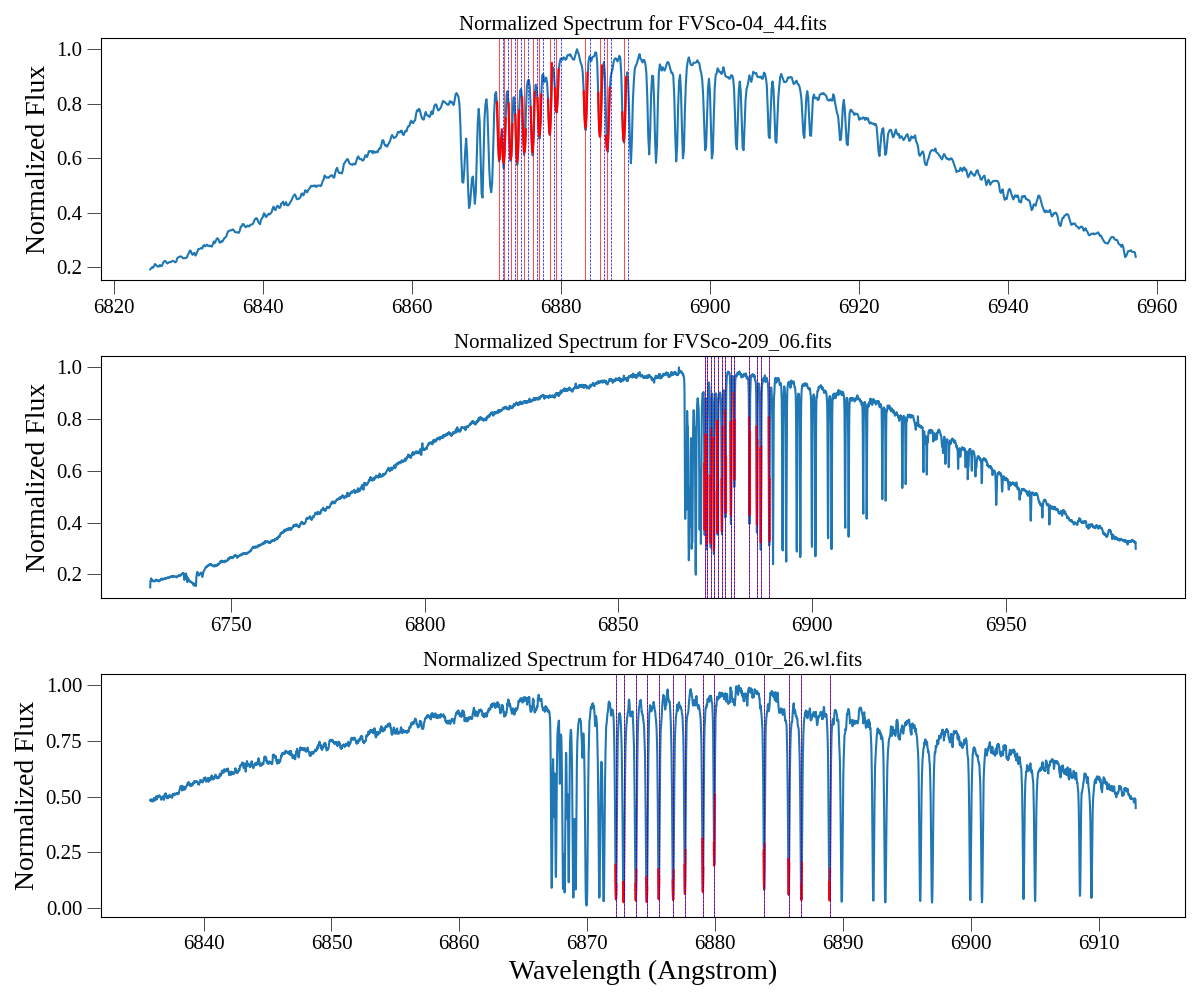
\includegraphics[width=1\textwidth]{spectra.png}
        \caption{Normalizovaná FVSco-04\_44.fits, FVSco-209\_06.fits a HD64740\_010r\_26.wl.fits}
        \label{fig:spectra}
    \end{figure*}

    \begin{figure*}
        \centering
        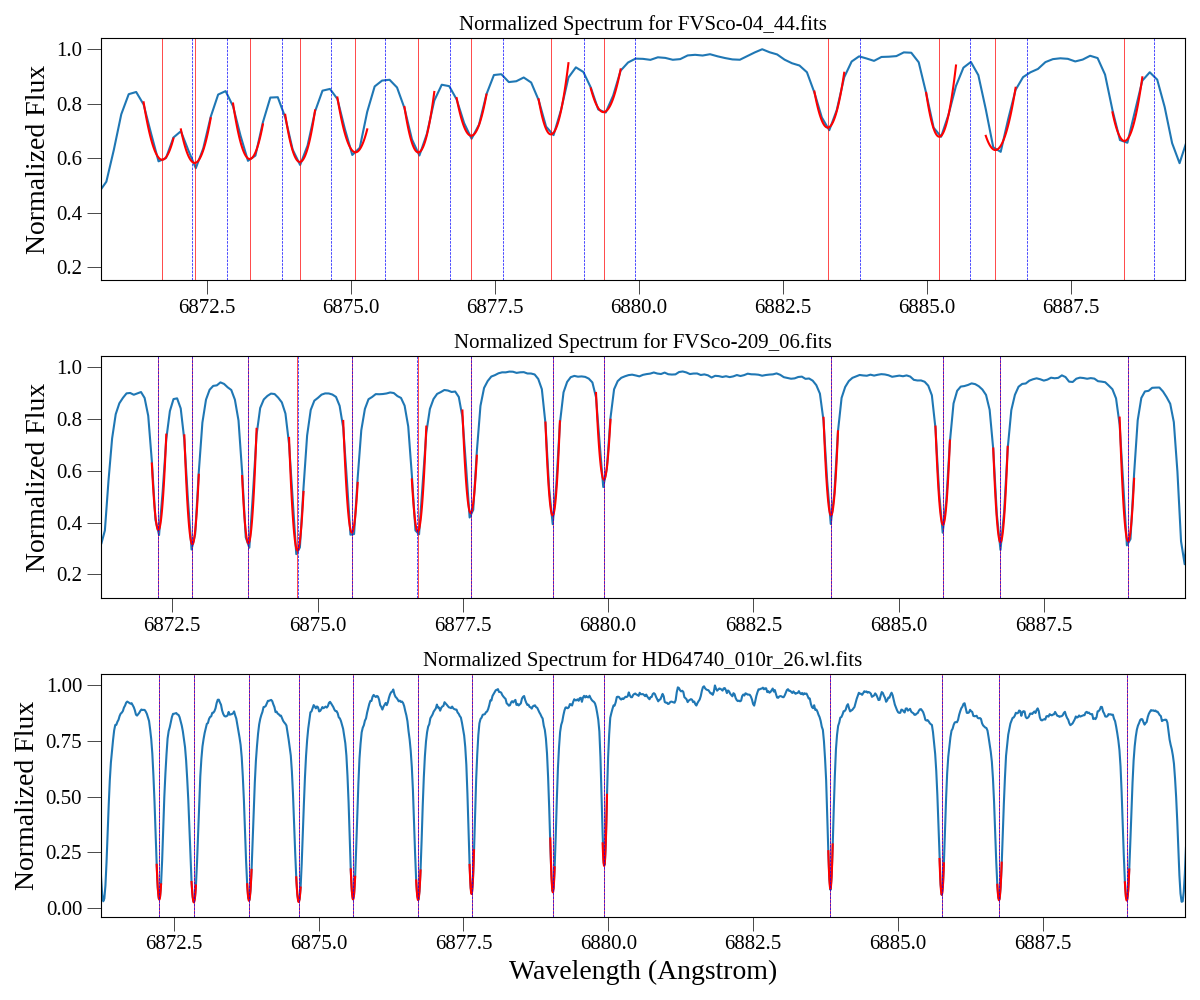
\includegraphics[width=1\textwidth]{spectra_telur.png}
        \caption{Část spektra použitá pro analýzu}
        \label{fig:spectra_telur}
    \end{figure*}

    \begin{figure*}
        \centering
        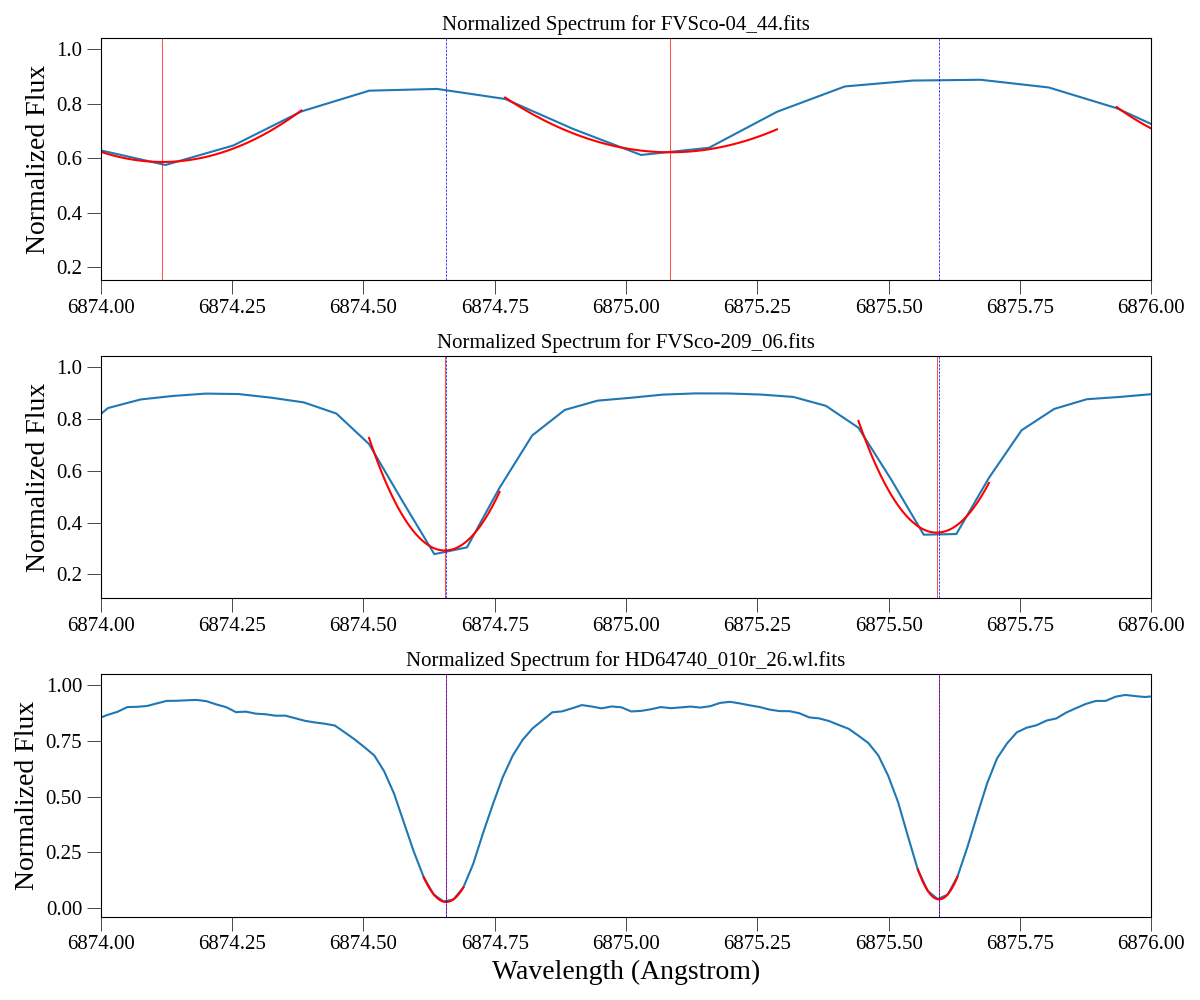
\includegraphics[width=1\textwidth]{spectra_lines.png}
        \caption{Fitování absorpčních čar}
        \label{fig:spectra_lines}
    \end{figure*}

    \begin{figure*}
        \centering
        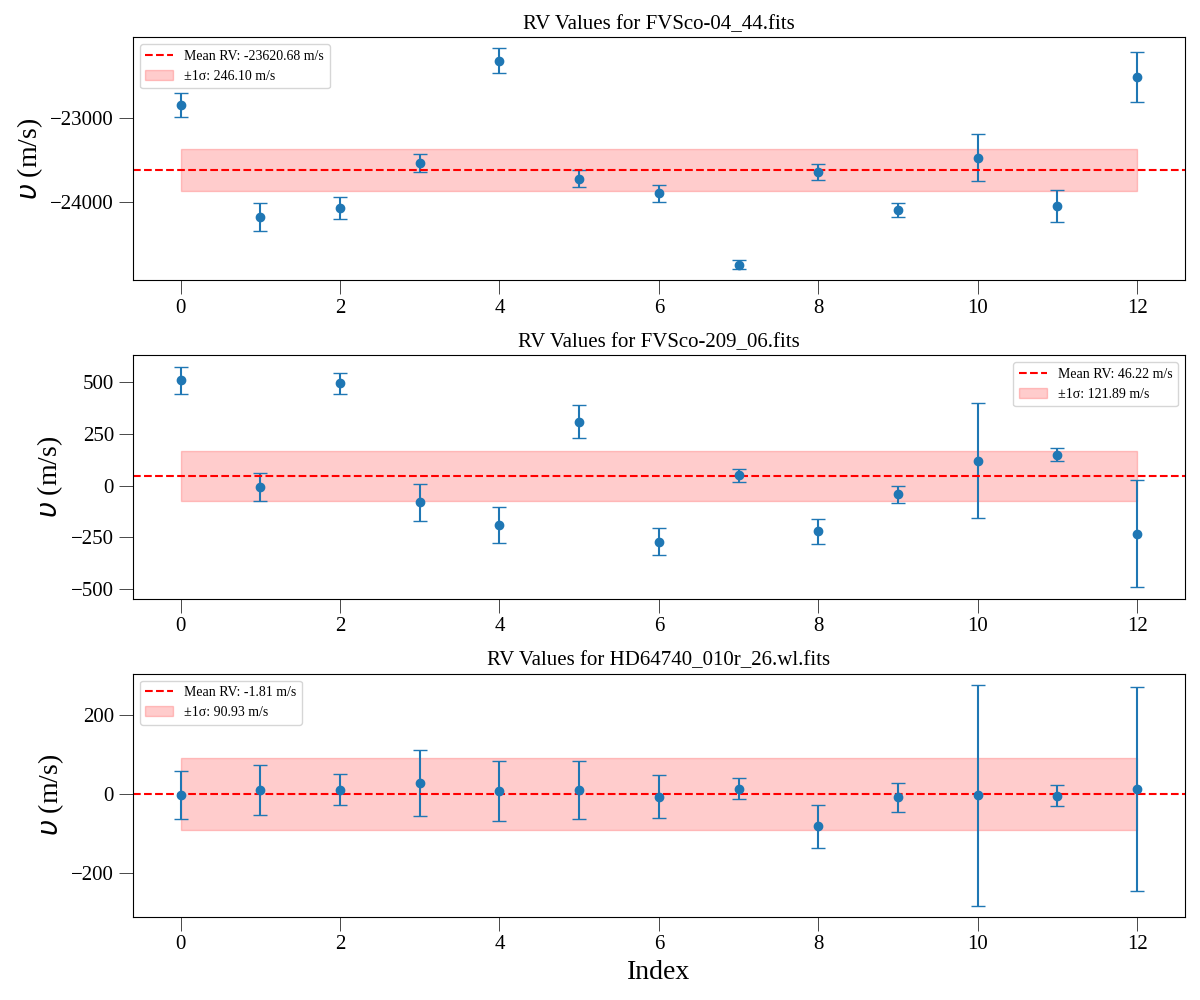
\includegraphics[width=1\textwidth]{rv_values.png}
        \caption{Radiální rychlosti pro jednotlivé čáry}
        \label{fig:rv_values}
    \end{figure*}

\end{document}